\chapter{Diskussion}

\glspl{can} sind ein wertvolles Werkzeug zur Transformation von Bildern einer Szene aus einer Ursprungsrepräsentation in eine Zielrepräsentation.
Diese Arbeit hat untersucht, ob sie sich auch für eine binäre Segmentierung im konkreten Fall einer Segmentierung von Kolorektalpolypen eignen.
Bei konsequenter Verwendung des CAN-Frameworks stellen sich die besten Ergebnisse mit einer Batch-Größe von 32 und einer Deaktivierung von Dropout zur Testzeit ein.
Geometrische Augmentierungen verbessern zwar die Ergebnisse auf den Trainings- und Validierungsdaten um bis zu 1,6 Prozentpunkte, verschlechtern allerdings die Ergebnisse auf den Testdaten um mindestens 11,5 Prozentpunkte.

Bei einem Training ohne GAN-Term und nur mit L1-Loss als Lerngrundlage stellen sich leicht bessere Ergebnisse auf den Trainingsdaten heraus.
Auf den Testdaten hingegen erreicht die kombinierte Verlustfunktion aus GAN-Term und L1-Loss leicht bessere Werte.
\citeauthor{Isola.2017} merken an, dass das \gls{can} bei der Multiklassen-Segmentierung viele kleine Objekte verschiedener Klassen detektiert, die in Wirklichkeit gar nicht da sind (s.~\autoref{fig:canseg}).
Dies lässt sich leider auch bei der binären Segmentierung beobachten wie bspw. in \autoref{fig:outputsb03}.

Interessanterweise weist ein Umkehren der Lernrichtung von Anfang ein stabileres Lernverhalten auf.
All dies lässt die Vermutung zu, dass reichhaltige Zielrepräsentationen eine Voraussetzung für ein stabiles Training von \glspl{can} sind.
Demnach sind \glspl{can} in ihrer bisherigen Form noch nicht das optimale Mittel, um eine binäre Segmentierung lernen zu lassen.

Das Verbesserungspotenzial ist sehr wahrscheinlich noch nicht ausgeschöpft.
Im folgenden werden weitere Möglichkeiten zur Verbesserung und Stabilisierung der \glspl{can} erörtert:

\glspl{gan} sind generell sehr sensitiv hinsichtlich der Wahl ihrer Hyperparameter.
Man könnte deshalb zur Verbesserung des Netzes generell oder zur besseren Anpassung auf das konkrete Problem der binären Segmentierung eine stratifizierte oder zufällige Suche der Trainingsparameter durchführen, um eine bessere Konstellation als die bereitgestellten Standardparameter (s.~\autoref{tab:train_def_val}) zu finden.
Aus zeitlichen Gründen konnte eine solche Suche im Rahmen dieser Arbeit nicht stattfinden.



\section{Verschwindende Gradienten}

\glspl{gan} haben außerdem oftmals mit Instabilität durch entweder explodierende oder verschwindende Gradienten zu kämpfen.
Dieses Problem tritt auch bei den \glspl{can} für binäre Segmentierung in Form von verschwindenden Gradienten auf (s.~\autoref{sec:batchsize}).
\citeauthor{Arjovsky.2017} zeigen auf, dass das Hinzufügen von Rauschen in der ersten Schicht des Diskriminators sowohl gegen verschwindende als auch explodierende Gradienten theoretisch ein gutes Mittel ist~\cite{Arjovsky.2017}.

Dies liegt darin begründet, dass im Falle von generativen Netzen die Region mit hoher Wahrscheinlichkeitsdichte der Verteilung des Generators und die des Diskriminators sich auf getrennten niedrigdimensionalen Mannigfaltigkeiten befinden, die nie perfekt zueinander ausgerichtet sind.
Andere generative Ansätze als die \glspl{gan} nutzen traditionellerweise Maximum-Likelihood-Schätzung zur Annäherung der beiden Verteilungen aneinander; dies entspricht der nicht-kommutativen \gls{kld}.
Liegen die beiden Verteilungen sehr weit voneinander entfernt, gibt die \gls{kld} dem Generator zu wenig Feedback, um lernen zu können.

Trainiert man den Diskriminator getrennt vom Generator auf optimale Bewertung, dann führt auch die originale Formulierung der \glspl{gan} für die Fake-Bewertung $ \mathbb{E}[\log(1 - D(G(\mathbf{z})))] $ dazu, dass der Gradient für den Generator fast überall Null wird.
Die alternative Formulierung des Generator-Terms mit $ \mathbb{E}[-\log(D(G(\mathbf{z})))] $ aus dem GAN-Paper~\cite{Goodfellow.2014} führt bei optimalem Diskriminator hingegen zu explodierenden Gradienten.

Fügt man jedoch Rauschen am Input des Diskriminators hinzu und nimmt die originale Formulierung des Generator-Terms, glättet man dessen Verteilung und sorgt somit dafür, dass der Gradient für den Generator der \gls{jsd} entspricht.
Diese Divergenz ist der Mittelwert der \glspl{kld} beider Verteilungskombinationen und nicht überall Null, selbst wenn beide Verteilungen weiter voneinander entfernt sind.
Somit kann ein solches Rauschen zumindest in der Theorie zu stabilen Gradienten führen, die weder verschwinden noch explodieren.
Die \glspl{can} von \citeauthor{Isola.2017} müssten dementsprechend so angepasst werden, dass sowohl Inputs als auch Targets mit einem Gauss'schen Rauschen gefiltert werden, bevor sie dem Diskriminator übergeben werden; der Generator hingegen erhält den originalen Datensatz.

Ein weiterer interessanter Ansatz basiert auf der Wasserstein-Distanz, welche die minimalen Kosten beim Transport aller Wahrscheinlichkeitsdichte einer Verteilung auf die Wahrscheinlichkeitsdichte einer anderen Verteilung ausdrückt~\cite{Arjovsky.2017}.
Wird ein Netz anhand dieser Metrik trainiert, approximiert der Diskriminator ebenfalls die \gls{jsd} und bietet damit dem Generator ständig Feedback zum Lernen.
Eine sehr vielversprechende Konsequenz dieses Aufbaus wäre, dass man tatsächlich zuerst den Diskriminator getrennt trainieren könnte bis zu einem optimalen Punkt und den Generator anschließend trainieren könnte, ohne befürchten zu müssen, dass der Diskriminator dem Generator zu wenig Feedback bietet.
Experimente hinsichtlich des Rhythmus von Diskriminator- und Generator-Updates bei den \glspl{can} könnten bei einer solchen Trainingsweise vermutlich entfallen.

Um ein \gls{wgan} zu implementieren, muss man die Wasserstein-Distanz allerdings approximieren, und dafür wird der Diskriminator durch einen "Kritiker" ersetzt, nämlich eine Funktion mit 1-Lipschitz-Stetigkeit~\cite{Arjovsky.2017b}.
Um diese Lipschitz-Stetigkeit der Funktion einzuhalten, wird im originalen Paper ein naives Begrenzen der Gewichte im Diskriminator mithilfe eines Hyperparameters umgesetzt.
Dies hält zwar die Lipschitz-Stetigkeit ein, begrenzt aber die Kapazität des Modells.
Durch eine Gradient Penalty, also eine Bestrafung von zu hohen Gradientenwerten, wird diese Situation wieder verbessert~\cite{Gulrajani.2017}.

\glspl{wgan} erreichen durchaus Ergebnisse, die ähnlich gut wie oder besser als traditionelle Architekturen wie \glspl{dcgan} sind, brauchen dafür aber in der Regel mehr Trainingszeit, wenn auch nicht mehr Iterationen.
Ihr großer Vorteil ist das deutlich stabilere Konvergieren, das ein Trainieren großer Netze besser möglich machen kann.
Außerdem erzielen \glspl{wgan} mit Gradient Penalty im Gegensatz zu vielen anderen erfolgreichen Architekturen selbst noch dann sehr gute Ergebnisse, wenn keinerlei Normalisierung in Generator und Diskriminator wie z.~B. in Form von Batch-Normalisierung geschieht oder wenn ein ResNet trainiert wird.



\section{Residual Learning}

Als eine sehr hilfreiche Taktik gegen explodierende oder verschwindende Gradienten hat sich bei Deep Learning neben Batch-Normalisierung auch \emph{Residual Learning} in Form von ResNets etabliert:
Statt nur die Anzahl an Schichten im Netz zu erhöhen, werden in wiederholenden Abständen parameterfreie Skip Connections mit elementweiser Summierung eingebaut, die nur eine Identität berechnen~\cite{He.2016}.
Dadurch lernen die dazwischen liegenden Schichten nur eine Restfunktion statt eine vollständige Funktion.
Ein "Baustein" im Rest-Lernen kann dann aussehen wie in \autoref{fig:resnetbuildingblock}.

\begin{figure}
	\centering
	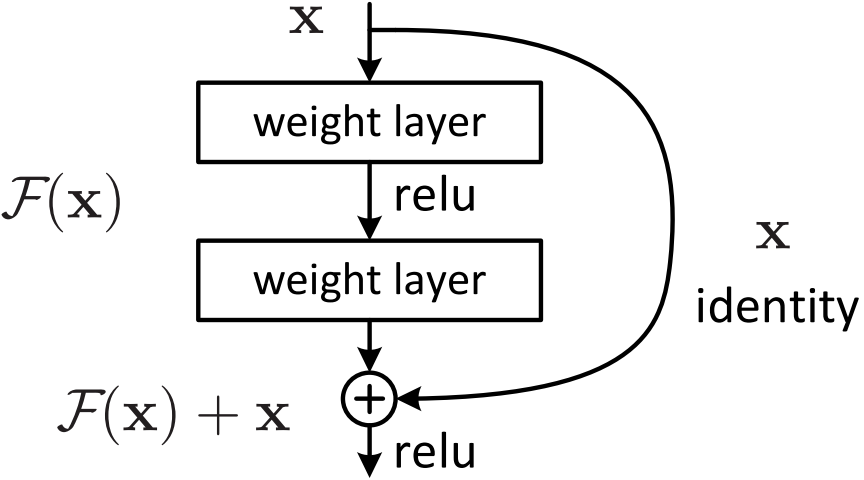
\includegraphics[width=0.5\linewidth]{img/resnet_building_block}
	\caption[Beispielhafter Baustein des ResNet]{Beispielhafter Baustein des ResNet~\cite{He.2016}}
	\label{fig:resnetbuildingblock}
\end{figure}

Bei der Objektdetektion und -lokalisierung in Bildern stellen die Autoren bei den ResNets deutliche Verbesserungen bei Steigerung der Netzfiefe fest im Gegensatz zu Referenzarchitekturen, bei denen eine Erhöhung der Tiefe eher noch eine Verschlechterung des Trainingsfehlers herbeiführt.
Erste Plätze bei Detektions- und Lokalisierungs-Challenges auf den Datasets ImageNet und COCO belegen die Wirksamkeit dieses Rest-Lernens.
Diesen Aufbau statt das U-Net als Grundlage für den Generator zu nehmen, könnte weitere Verbesserungen bei der Stabilisierung des Trainings bewirken.

Wie ein Segmentierungsnetz aussehen kann, das auf Rest-Lernen basiert, zeigen die \emph{RedNets} von \citeauthor{Mao.2016}~\cite{Mao.2016}.
Sehr gute Ergebnisse werden erzielt, wenn als Baustein zwei Ebenen aus Faltung, Rest-Lernen und Entfaltung gelernt werden (s.~\autoref{fig:rednetbuildingblock}).
Eine solche Architektur im Generator der \glspl{can} zu verwenden, könnte nicht nur zu besseren Ergebnissen, sondern auch zu besserer Stabilität im Training führen.

\begin{figure}
	\centering
	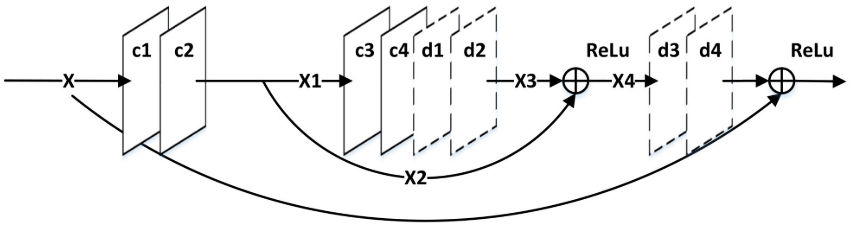
\includegraphics[width=0.8\linewidth]{img/rednet_building_block}
	\caption[Ein Baustein des RedNet]{Ein Baustein des RedNet~\cite{Mao.2016}. Kurven stehen für Skip Connections mit Identitätsmapping, voll umrandete Rechtecke für Faltungen (\emph{c1} etc.), gestrichelt umrandete für Entfaltungen (\emph{d1} etc.).}
	\label{fig:rednetbuildingblock}
\end{figure}



\section{Weiterentwicklungen der CANs}

Die Autoren der \glspl{can} haben ihren Ansatz bereits weiterentwickelt für eine Bild-zu-Bild-Übersetzung, bei der keine direkten Bild-zu-Bild-Paare zum Training zur Verfügung stehen~\cite{Zhu.2018}.
Stattdessen stehen eine \emph{Menge $ X $ an Inputs} einer \emph{Menge $ Y $ an Targets} gegenüber.
Mithilfe des GAN-Frameworks wird eine Projektion von $ X $ nach $ Y $ gelernt.
Diese wird mithilfe der Verlustfunktion auf Zyklenkonsistenz beschränkt, sodass nach einem Mapping von $ X $ nach $ Y $ das Mapping des Ergebnisses $ Y' $ auf $ X $ wieder ähnlich wie $ X $ sein muss.
Indem sie das GAN-Training mit einem Zyklenkonsistenz-Loss für beide Prädiktionsrichtungen kombinieren, übertreffen sie aktuelle Ansätze.
Für eine Multiklassen-Segmentierung verschlechtert sich allerdings das Ergebnis gegenüber den \glspl{can}.
